\documentclass[tikz,border=7pt]{standalone}

\usepackage[T1]{fontenc}
\usepackage[utf8]{inputenc}
\usepackage{amsfonts}
\usepackage{tikz}
\usetikzlibrary{arrows.meta, calc, fit, positioning}

\begin{document}

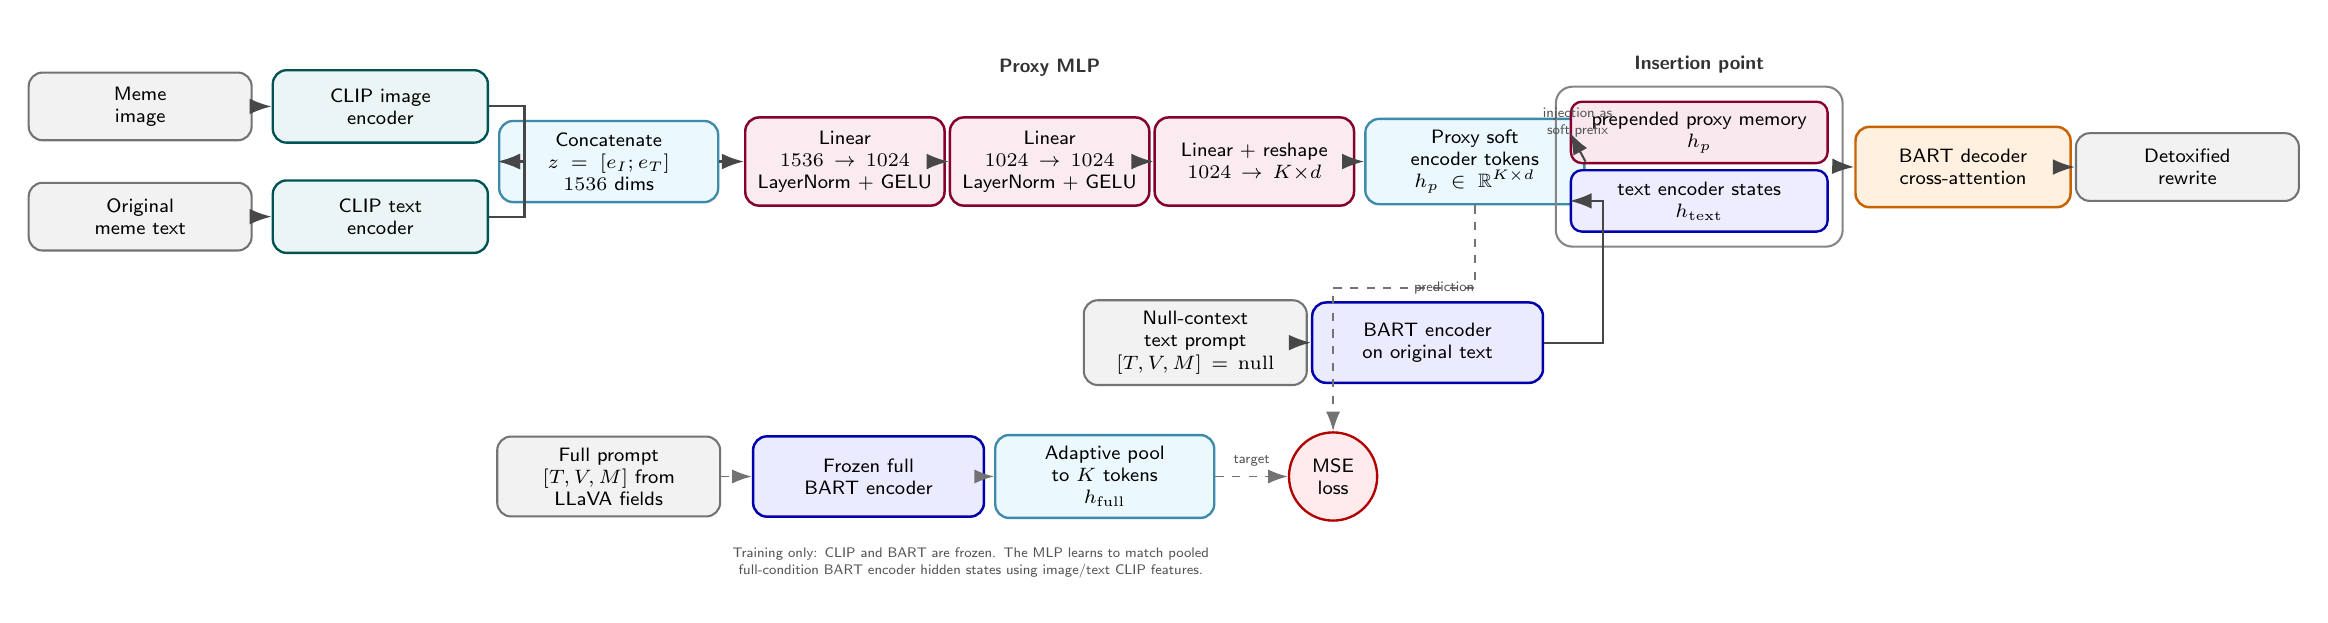
\begin{tikzpicture}[
    every node/.style={font=\sffamily},
    arrow/.style={-{Latex[length=2.8mm,width=2.0mm]}, line width=0.75pt, draw=black!72},
    trainarrow/.style={-{Latex[length=2.5mm,width=1.8mm]}, line width=0.65pt, draw=black!55, dashed},
    input/.style={
        rectangle,
        rounded corners=5pt,
        draw=black!55,
        fill=black!5,
        line width=0.75pt,
        align=center,
        text width=2.55cm,
        minimum height=0.86cm,
        inner sep=4pt,
        font=\sffamily\scriptsize
    },
    clip/.style={
        rectangle,
        rounded corners=5pt,
        draw=teal!65!black,
        fill=teal!8,
        line width=0.85pt,
        align=center,
        text width=2.45cm,
        minimum height=0.92cm,
        inner sep=4pt,
        font=\sffamily\scriptsize
    },
    embed/.style={
        rectangle,
        rounded corners=5pt,
        draw=cyan!65!black,
        fill=cyan!8,
        line width=0.85pt,
        align=center,
        text width=2.50cm,
        minimum height=1.03cm,
        inner sep=4pt,
        font=\sffamily\scriptsize
    },
    mlp/.style={
        rectangle,
        rounded corners=5pt,
        draw=purple!70!black,
        fill=purple!8,
        line width=0.9pt,
        align=center,
        text width=2.25cm,
        minimum height=1.12cm,
        inner sep=4pt,
        font=\sffamily\scriptsize
    },
    bart/.style={
        rectangle,
        rounded corners=5pt,
        draw=blue!68!black,
        fill=blue!8,
        line width=0.9pt,
        align=center,
        text width=2.65cm,
        minimum height=1.02cm,
        inner sep=4pt,
        font=\sffamily\scriptsize
    },
    decoder/.style={
        rectangle,
        rounded corners=5pt,
        draw=orange!78!black,
        fill=orange!12,
        line width=0.9pt,
        align=center,
        text width=2.45cm,
        minimum height=1.02cm,
        inner sep=4pt,
        font=\sffamily\scriptsize
    },
    memoryproxy/.style={
        rectangle,
        rounded corners=4pt,
        draw=purple!70!black,
        fill=purple!9,
        line width=0.85pt,
        align=center,
        text width=3.05cm,
        minimum height=0.78cm,
        inner sep=3pt,
        font=\sffamily\scriptsize
    },
    memorytext/.style={
        rectangle,
        rounded corners=4pt,
        draw=blue!68!black,
        fill=blue!7,
        line width=0.85pt,
        align=center,
        text width=3.05cm,
        minimum height=0.78cm,
        inner sep=3pt,
        font=\sffamily\scriptsize
    },
    loss/.style={
        circle,
        draw=red!70!black,
        fill=red!8,
        line width=0.85pt,
        align=center,
        minimum size=1.12cm,
        inner sep=1pt,
        font=\sffamily\scriptsize
    },
    label/.style={font=\sffamily\tiny, align=center, text=black!68},
    section/.style={font=\sffamily\bfseries\scriptsize, align=center, text=black!80}
]

\path[fill=white] (-1.05,-4.95) rectangle (27.35,2.25);

% ---------------------------------------------------------------------------
% Inference path: CLIP -> proxy MLP -> BART encoder memory -> decoder.
% ---------------------------------------------------------------------------
\node[input] (image) at (0.0, 1.25) {Meme\\image};
\node[input] (text) at (0.0,-0.15) {Original\\meme text};

\node[clip] (clipimage) at (3.05, 1.25) {CLIP image\\encoder};
\node[clip] (cliptext) at (3.05,-0.15) {CLIP text\\encoder};

\node[embed] (features) at (5.95, 0.55) {Concatenate\\$z=[e_I;e_T]$\\$1536$ dims};

\node[mlp] (mlp1) at (8.95, 0.55) {Linear\\$1536 \rightarrow 1024$\\LayerNorm + GELU};
\node[mlp] (mlp2) at (11.55, 0.55) {Linear\\$1024 \rightarrow 1024$\\LayerNorm + GELU};
\node[mlp] (mlp3) at (14.15, 0.55) {Linear + reshape\\$1024 \rightarrow K{\times}d$};
\node[embed] (softtokens) at (16.95, 0.55) {Proxy soft\\encoder tokens\\$h_p \in \mathbb{R}^{K\times d}$};

\node[input] (noneprompt) at (13.40,-1.75) {Null-context\\text prompt\\$[T,V,M]=\mathrm{null}$};
\node[bart] (textencoder) at (16.35,-1.75) {BART encoder\\on original text};

\node[memoryproxy] (proxymem) at (19.80, 0.92) {prepended proxy memory\\$h_p$};
\node[memorytext] (textmem) at (19.80, 0.05) {text encoder states\\$h_{\mathrm{text}}$};
\node[
    rectangle,
    rounded corners=6pt,
    draw=black!48,
    line width=0.75pt,
    inner sep=5pt,
    fit=(proxymem)(textmem),
    label={[label]above:BART encoder memory}
] (memorybox) {};

\node[decoder] (decoder) at (23.15, 0.48) {BART decoder\\cross-attention};
\node[input] (rewrite) at (26.00, 0.48) {Detoxified\\rewrite};

\draw[arrow] (image) -- (clipimage);
\draw[arrow] (text) -- (cliptext);
\draw[arrow] (clipimage.east) -- ++(0.45,0) |- (features.west);
\draw[arrow] (cliptext.east) -- ++(0.45,0) |- (features.west);
\draw[arrow] (features) -- (mlp1);
\draw[arrow] (mlp1) -- (mlp2);
\draw[arrow] (mlp2) -- (mlp3);
\draw[arrow] (mlp3) -- (softtokens);
\draw[arrow] (softtokens.east) -- node[above,label] {injection as\\soft prefix} (proxymem.west);

\draw[arrow] (noneprompt) -- (textencoder);
\draw[arrow] (textencoder.east) -- ++(0.75,0) |- (textmem.west);
\draw[arrow] (memorybox.east) -- (decoder.west);
\draw[arrow] (decoder) -- (rewrite);

\node[section] at (11.55, 1.74) {Proxy MLP};
\node[section] at (19.80, 1.78) {Insertion point};

% ---------------------------------------------------------------------------
% Training-only target path used to supervise the proxy.
% ---------------------------------------------------------------------------
\node[input] (fullprompt) at (5.95,-3.45) {Full prompt\\$[T,V,M]$ from\\LLaVA fields};
\node[bart] (fullencoder) at (9.25,-3.45) {Frozen full\\BART encoder};
\node[embed] (pool) at (12.25,-3.45) {Adaptive pool\\to $K$ tokens\\$h_{\mathrm{full}}$};
\node[loss] (mseloss) at (15.15,-3.45) {MSE\\loss};

\draw[trainarrow] (fullprompt) -- (fullencoder);
\draw[trainarrow] (fullencoder) -- (pool);
\draw[trainarrow] (pool) -- node[above,label] {target} (mseloss);
\draw[trainarrow] (softtokens.south) -- ++(0,-1.05) -| node[pos=0.25,right,label] {prediction} (mseloss.north);

\node[label, text width=9.0cm] at (10.55,-4.55) {
Training only: CLIP and BART are frozen. The MLP learns to match pooled
full-condition BART encoder hidden states using image/text CLIP features.
};

\end{tikzpicture}

\end{document}
